\documentclass[letter]{ourGreenwayBrand}

\headerlabel{Research Brief}

\titletext{Once We Get There: A Plethora Of Parks - Utopía De Iztapalapa Atzintli}
\subtitletext{A plethora of parks: how vibrant urban spaces pay for themselves}
\authortext{Diana Guzman Porras}
\editedtext{Jack Lawson}
\datetext{August 16, 2025}

\begin{document}
\MakeBrandTitle

\section{Introduction}
Micromobility and infrastructure development are core focuses of Our Greenway, but in both cases they are means to equitable ends. Strong micromobility options make life easier and more enjoyable, not to mention more affordable. Providing citizens with a diversity of well-funded choices is preferable to having to find ways to afford the only option available.

With all this in mind, one of our biggest goals as a team is to showcase examples of this tied to place, activity, and access. Discovering our urban environments through exploration and play are key aspects of city life that Our Greenway seeks to strengthen.

The multi park projectUtopias de Iztapalapa\footnote{\url{https://www.utopiasiztapalapa.com/}}is one such example of a park system that aligns Our Greenway’s revitalization goals.

\begin{figure}[htbp]
  \centering
  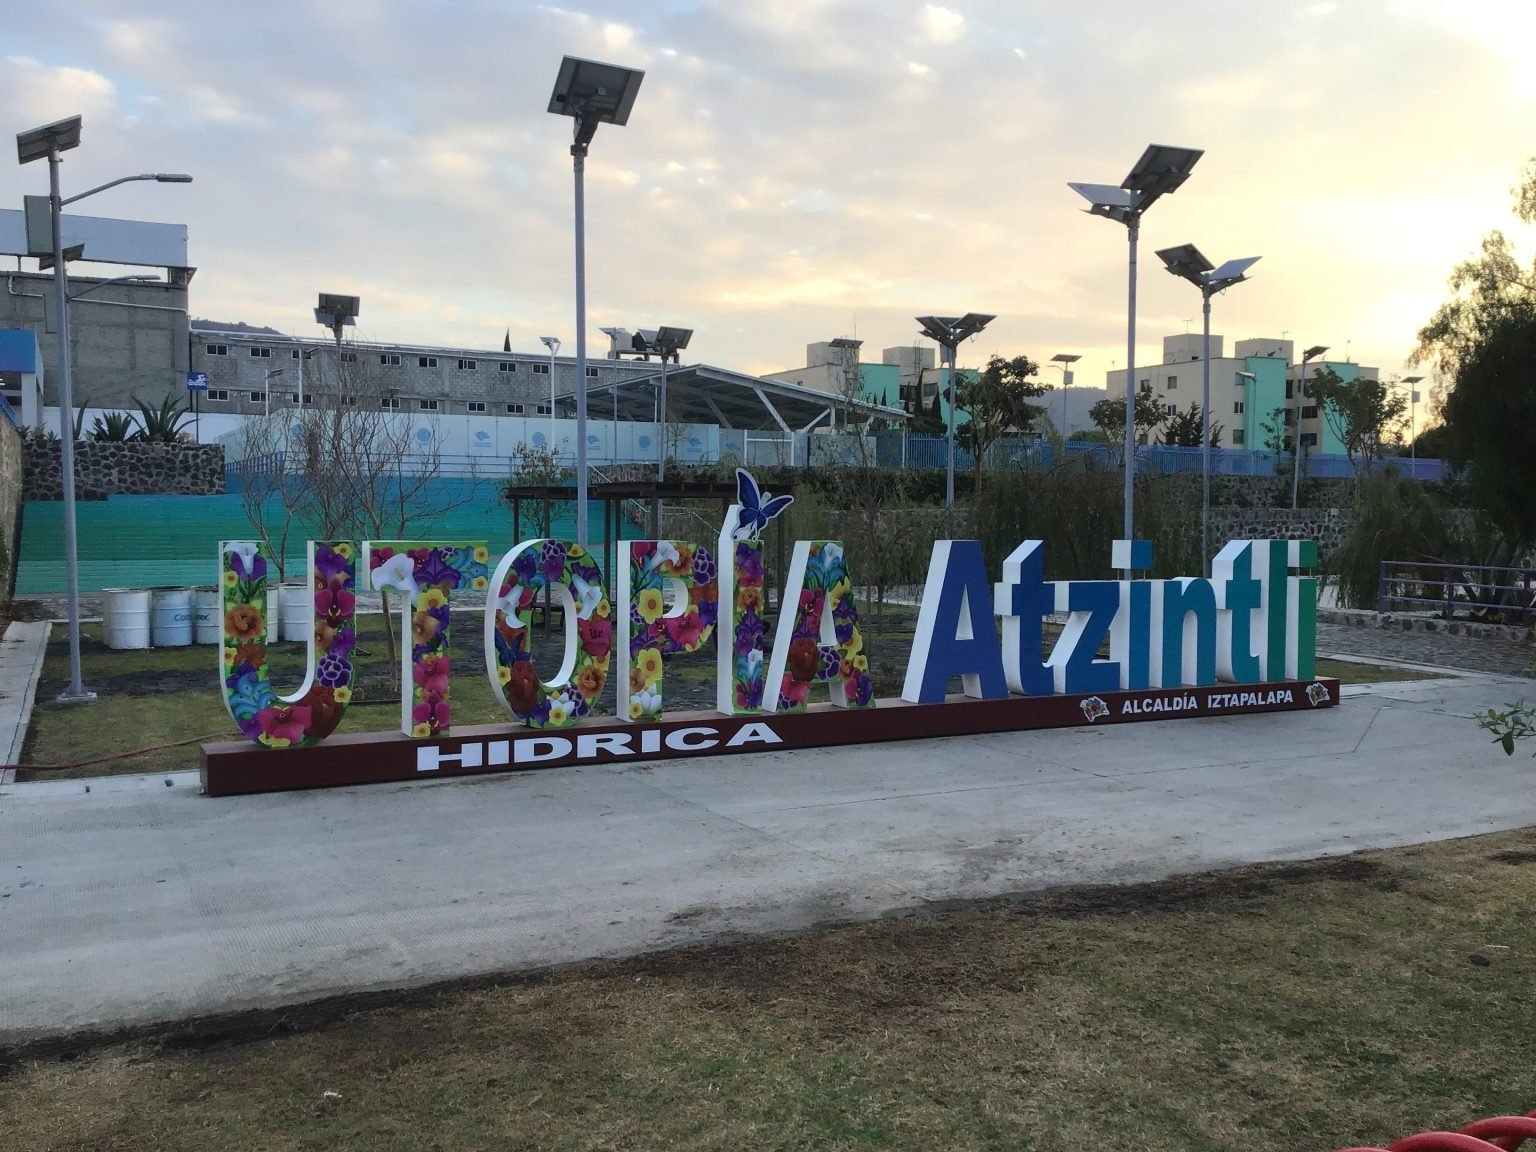
\includegraphics[width=0.7\textwidth]{images/IMG_8088-1536x1152.jpg}
\end{figure}

During our most recent research trip to Mexico one of the destinations we had to check out was the “new” cableway line installed in the Iztapalapa municipality.

Iztapalapa is largely known for its problems with water distribution infrastructure, overpopulation, and insecurity. Our main interest was to understand why they would opt for a cableway line as the best option for the mobility problems this place was facing. However, once we saw the Utopia park it became clear that the answer was not only in the transportation system they had chosen, but rather that it was simply part of the planning process.

\begin{figure}[htbp]
  \centering
  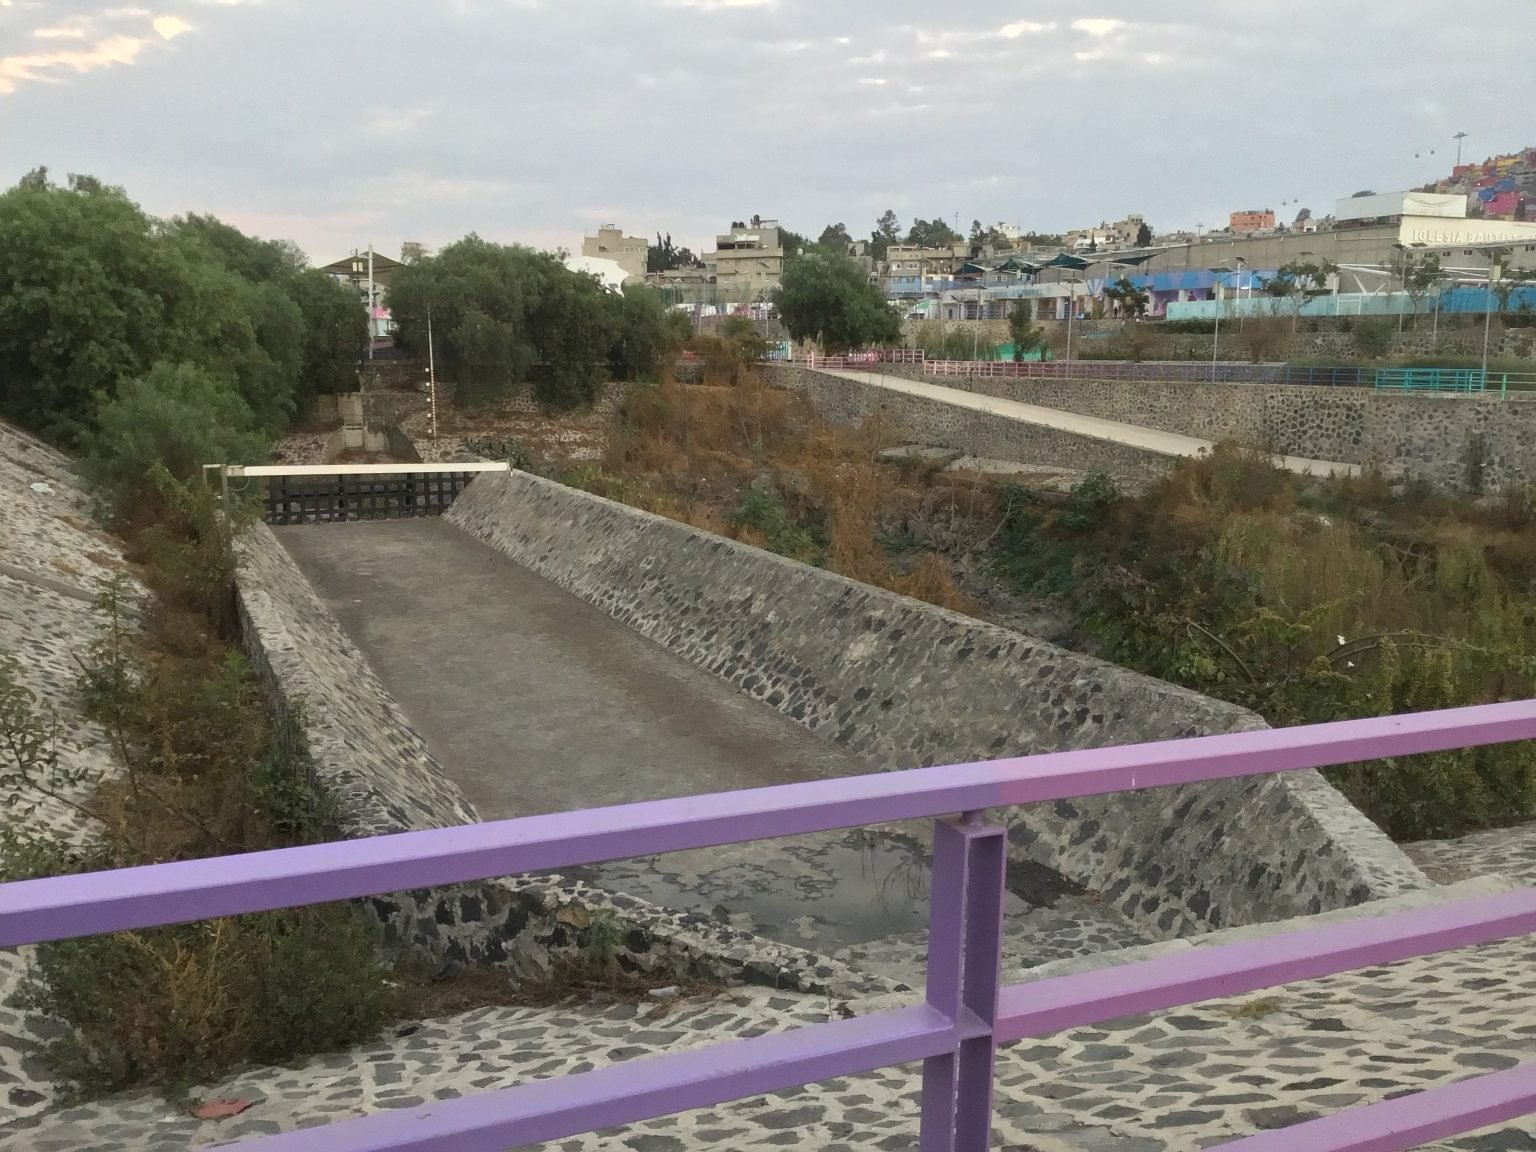
\includegraphics[width=0.7\textwidth]{images/IMG_8120-1536x1152.jpg}
\end{figure}

The park Utopia, as well as a good portion of the Iztapalapa municipality, are located on the Cerro de la Estrella, which means you are either going uphill or downhill at all times. The streets are narrow, occupied by large public buses in different states of disrepair, or by parked cars – some of which are in the middle of DIY repairs . We could only imagine the stress these streets were under with almost two million people  trying to meet their mobility needs.

What made us set our sights on the Park Utopía was learning that it was a park with the double purpose of A) providing a safe public space for integration and B) to contribute to the water management solution. This was the first time we had found a hybridized approach in Mexico.  We were intrigued.

\begin{figure}[htbp]
  \centering
  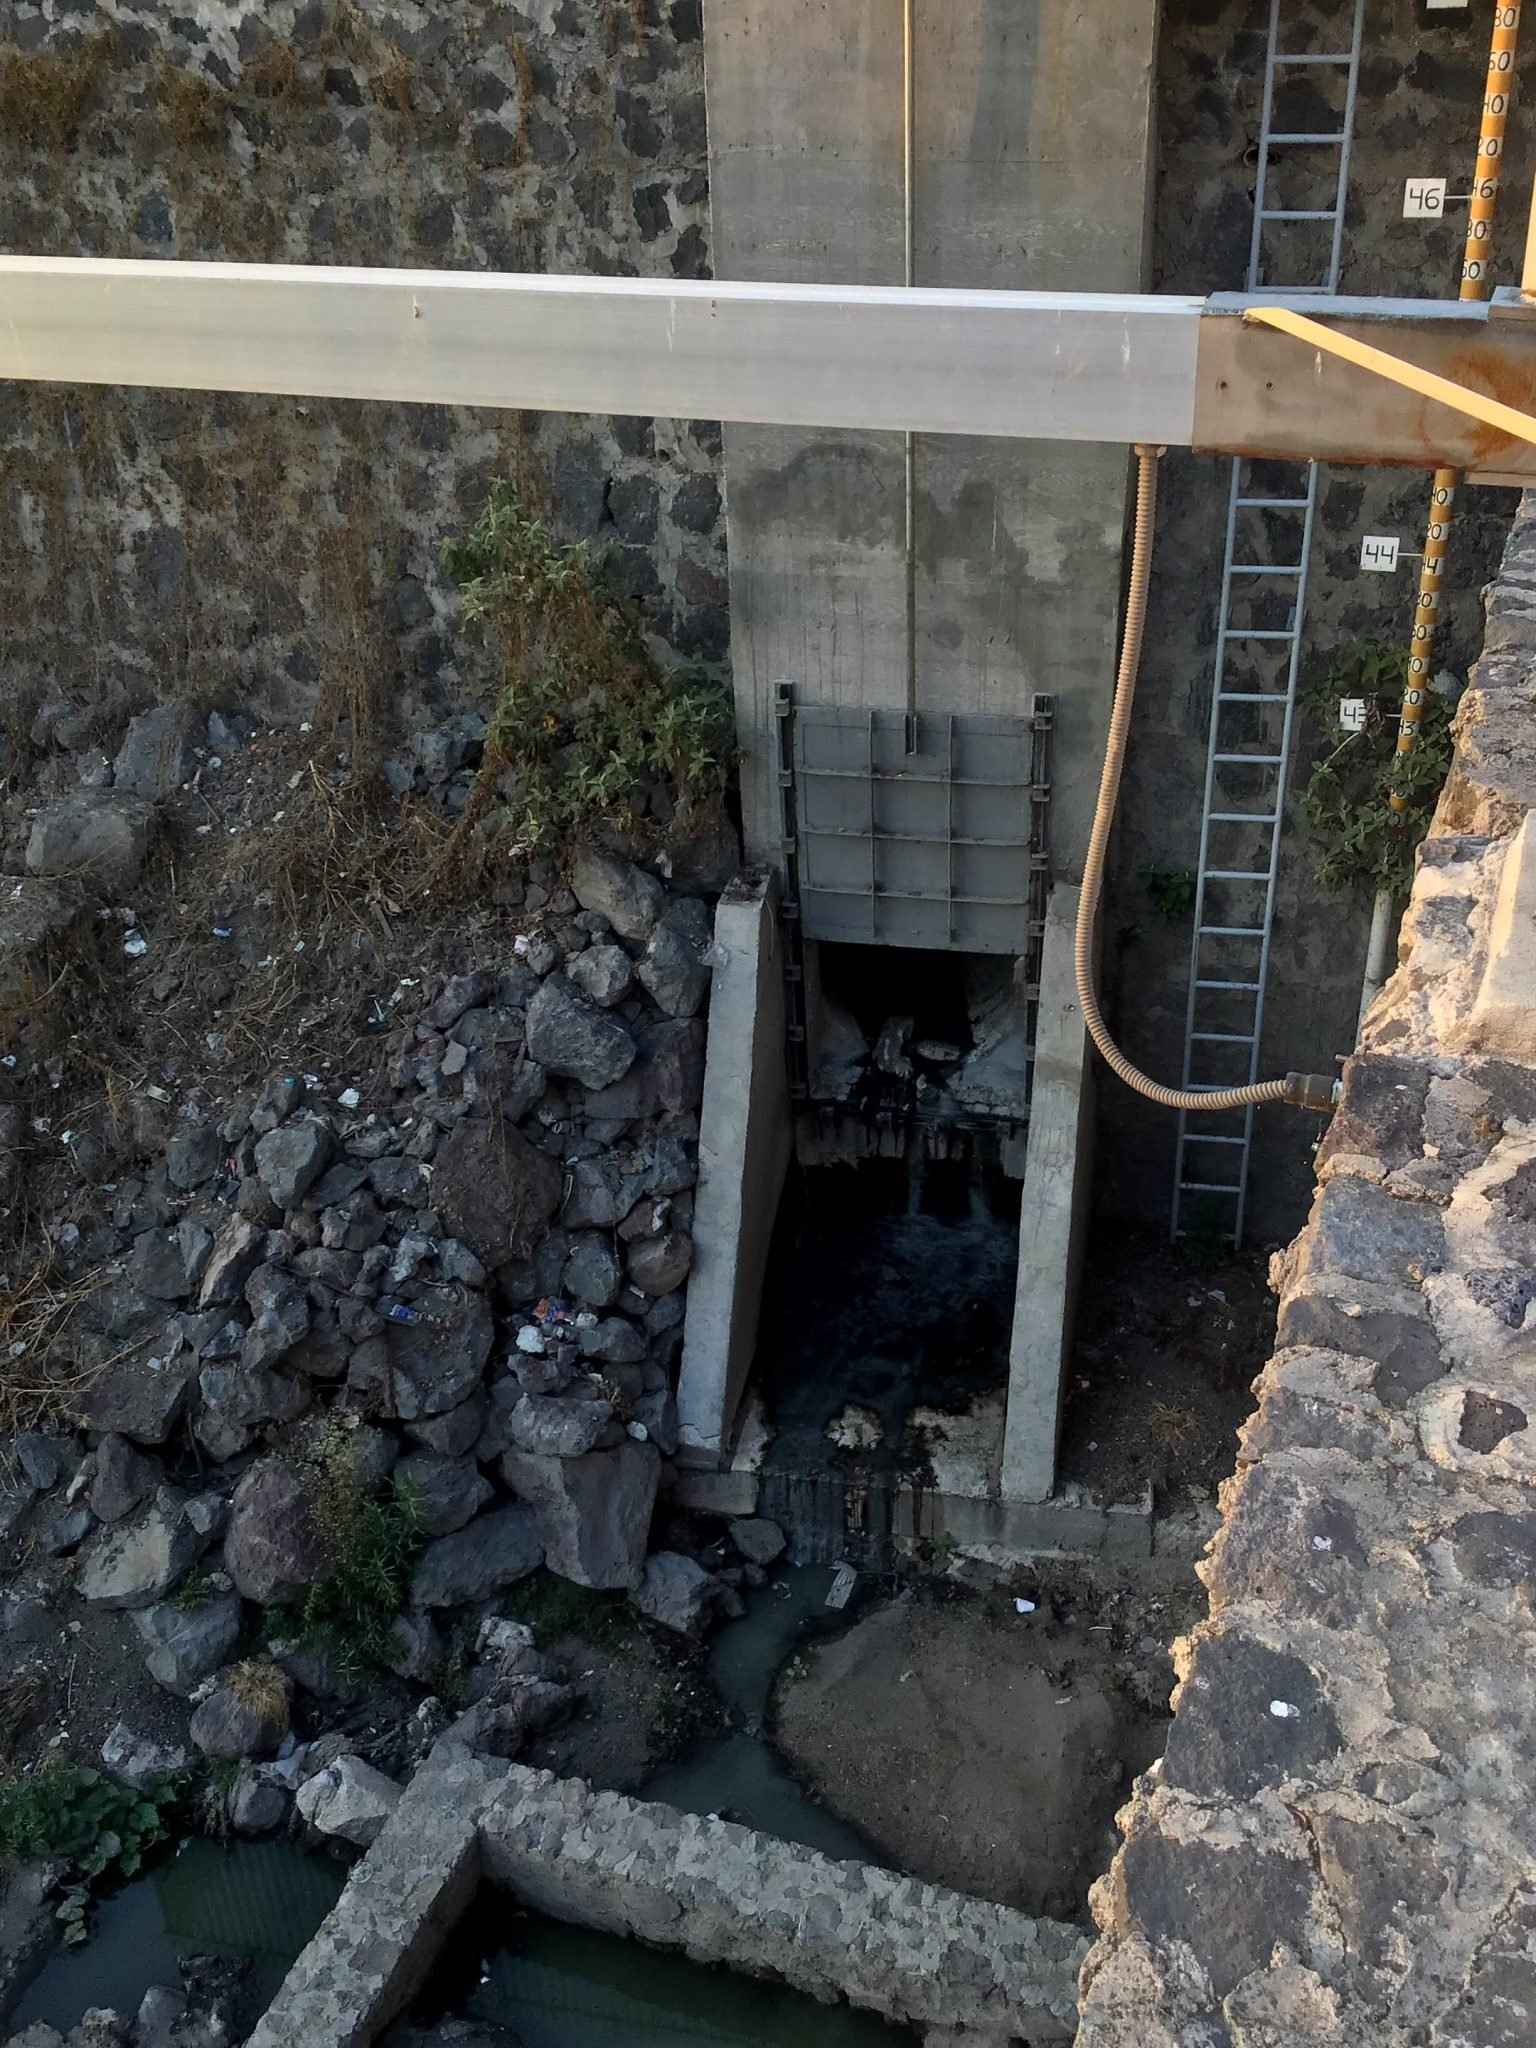
\includegraphics[width=0.7\textwidth]{images/IMG_8074-1536x2048.jpg}
\end{figure}

The first time we went to this park, we took a taxi from Coyoacán, which lies in southeast Mexico City, to the southwest. Not knowing the roads, time necessary to make it there, and still having a respectful fear of the ongoing pandemic, we decided a private car was a better choice that transit. And I’m glad for it, because otherwise it would have not been so evident why a cableway was indeed the way to go.

Upon arrival we felt safe. The park is big for Mexico City standards, with almost 36,500 square meters it is one of the biggest parks that isn’t regarded as a forest. According to Arquine , the water recollection system has the capacity to treat one liter of water per second through a dual system of activated mud and artificial wetlands. The system collects water from the adjacent streets and mitigates the risk of flooding. And the treated water is used to keep the park and serve the community.  The really unique aspect of this is that the system was right there for anyone to look at – and this visibility seemed to encourage local people to learn about it.

\begin{figure}[htbp]
  \centering
  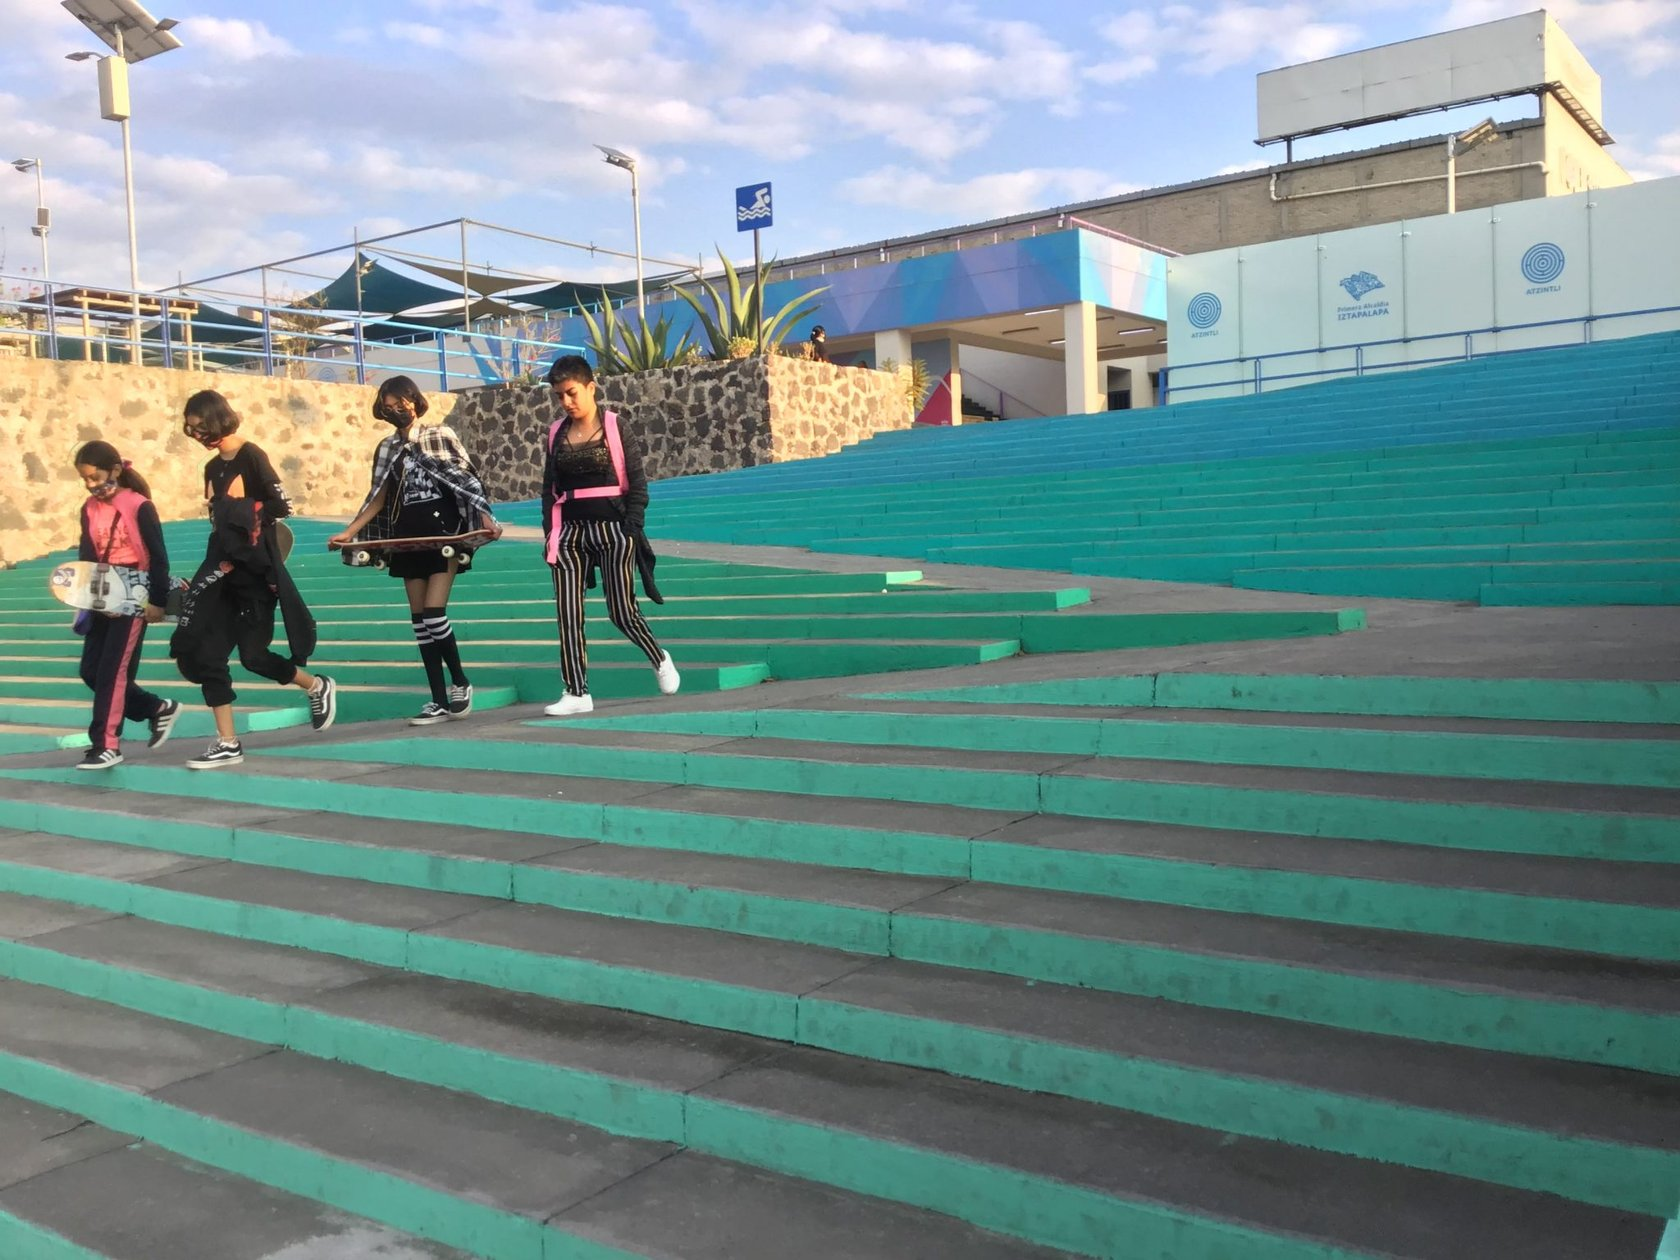
\includegraphics[width=0.7\textwidth]{images/IMG_8012-2048x1536.jpg}
\end{figure}

As we kept walking several things caught our attention, the first was the immediate sense of integration the park promoted.  They had chosen ramps over stairs in most situations, which were big enough to allow the usage of wheelchairs, strollers or skateboards – possibly even at the same time.

They even used ramps within staircases – which raised a safety question for us, since those can be deemed dangerous in Canada due to visibility mainly during winter or rainy weather – but we still found it interesting, and the park users seemed to navigate it easily.

\begin{figure}[htbp]
  \centering
  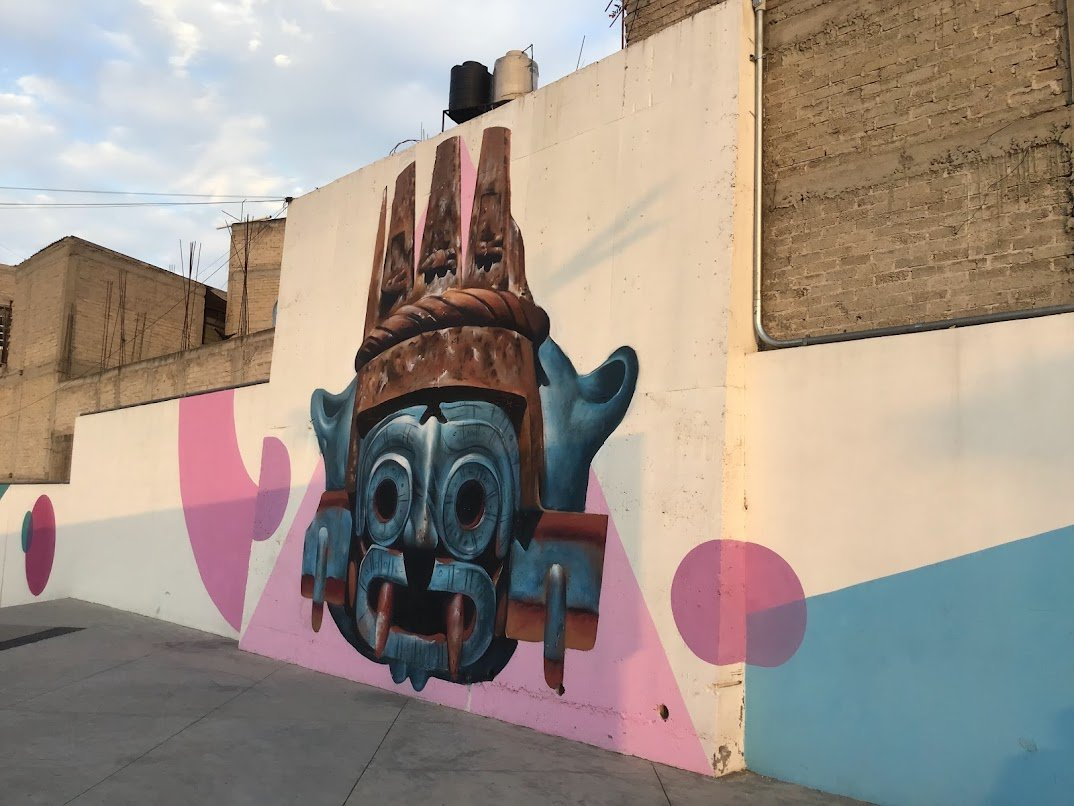
\includegraphics[width=0.7\textwidth]{images/Untitled-1.png}
\end{figure}

The color scheme of the park was dominated by the gray of the cement, but with bursts of green from the trees and plants. Decorations and street art were in shades of  purple and yellow followed by unconventional tones of pink and blue in paint.

Murals depicting cultural aspects of Mexican tradition made it clear that this was not a place designed for disenfranchisment and discrimination. This was partly accomplished through the recognition of non-traditional sports or artistic activities such as skateboarding and graffiti.

We visited the activities center and were invited to their weekly chess class.  Once we had respectfully declined, we were left alone to explore at will. The center offers activities of all sorts, from music, to dance, to theater, poetry, drawing, and more.

With that said, the one thing that blew us away was a series of seminars to guide people in connecting with older members of their community. A big poster placed at the center of the wall explained (in Spanish of course)  why it could be difficult to find common ground with elders or youth while offering a place to learn to communicate better with them.

\begin{figure}[htbp]
  \centering
  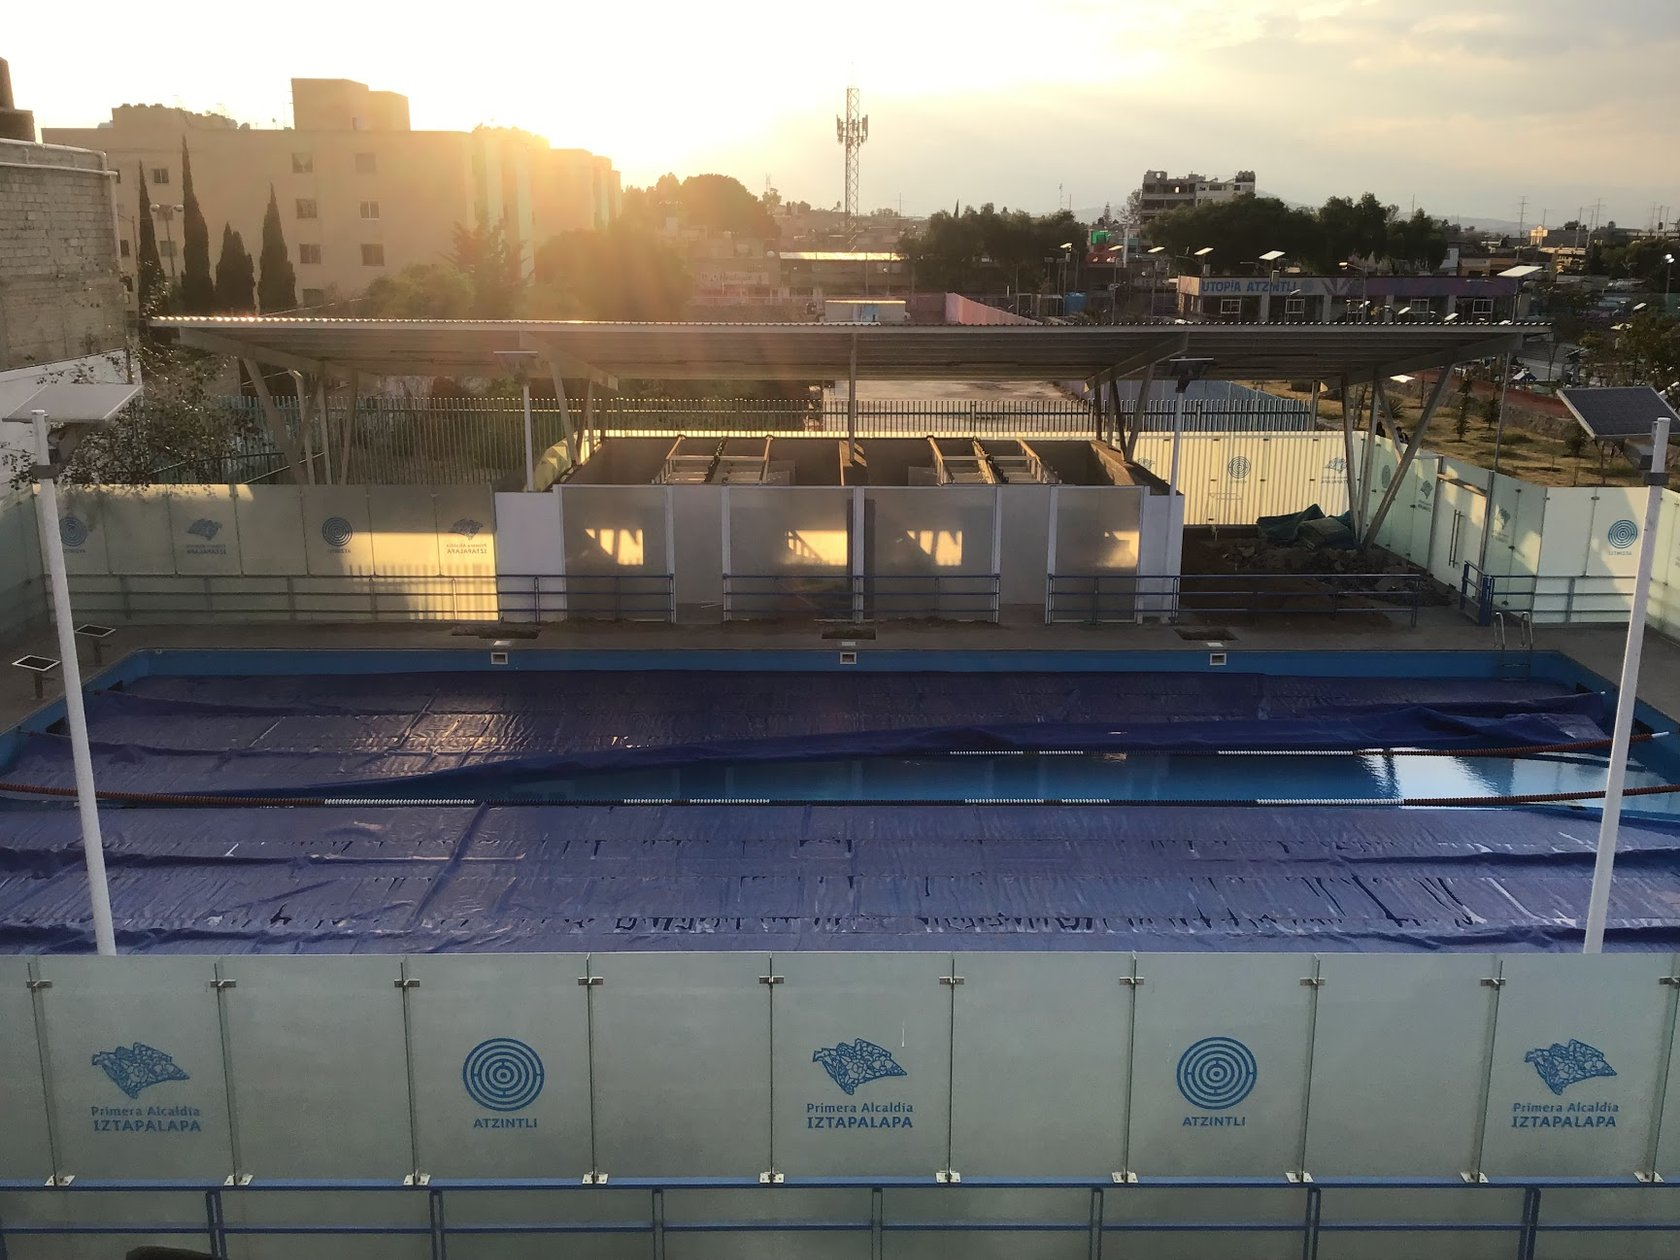
\includegraphics[width=0.7\textwidth]{images/Untitled_copy.png}
\end{figure}

The sports installations also promoted both team and individual efforts. The courts worked for both soccer and basketball, ensuring that with as little as one ball many people could enjoy recreation and social activity. There were also both skateboarding ramps, and  padded track circuits.

However, it was the  semi Olympic sized public pool that caught our attention. Given that Iztapalapa is known for its water problems, the opportunity to engage in recreational activities that include water are scarce.

\begin{figure}[htbp]
  \centering
  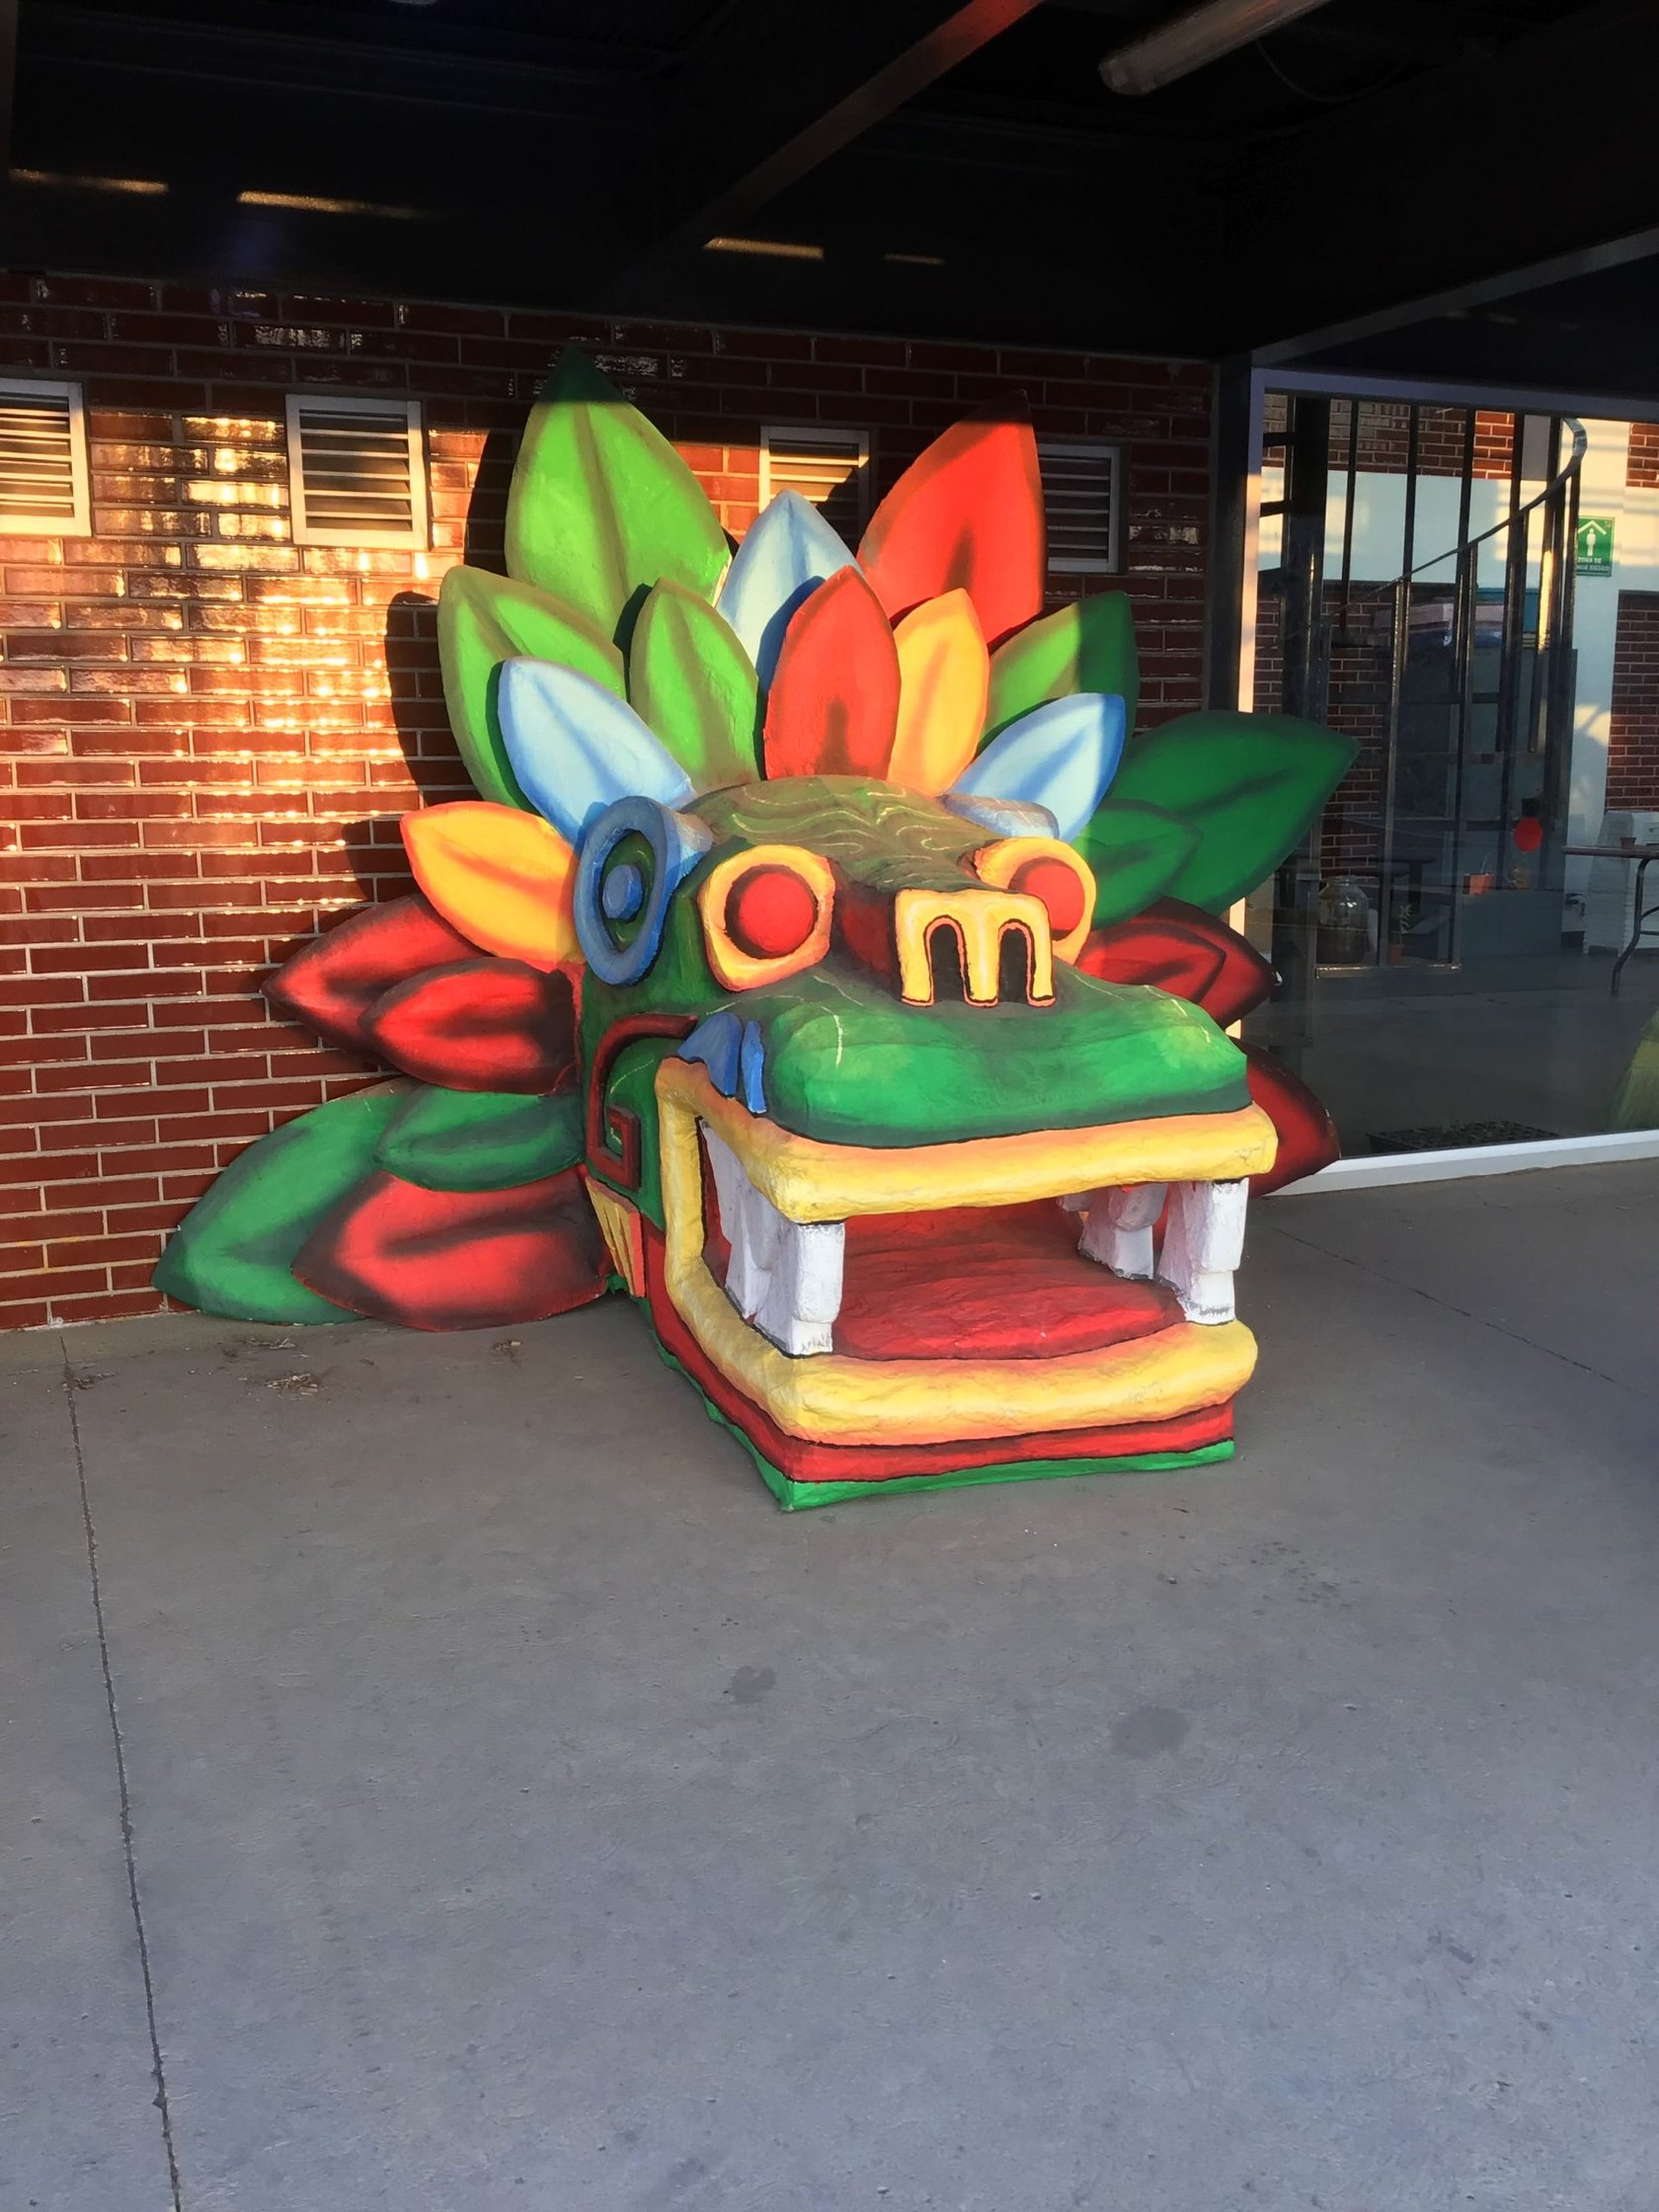
\includegraphics[width=0.7\textwidth]{images/IMG_8064-scaled.jpg}
\end{figure}

As our last observation we examined the little details surrounding a water recollection park.

Almost every aspect of Utopia Atzintli’s layout was designed to redirect the water to the collecting pond. Every ramp, nook and channel worked in favor of this. This turned the park into not only a piece of structural infrastructure, but an educational opportunity as well. The diversity of programming also seemed to attract an inter-generational mix of people.

Never before had I seen a place where little children, kids, teenagers, young adults and grown adults shared space and actively participated in the same activities at the same time. Despite our visit occurring late during the day, and there being no signs regarding littering, nor cleaning crew, the park was completely clean. It was a pleasant surprise and an enjoyable experience.

\begin{figure}[htbp]
  \centering
  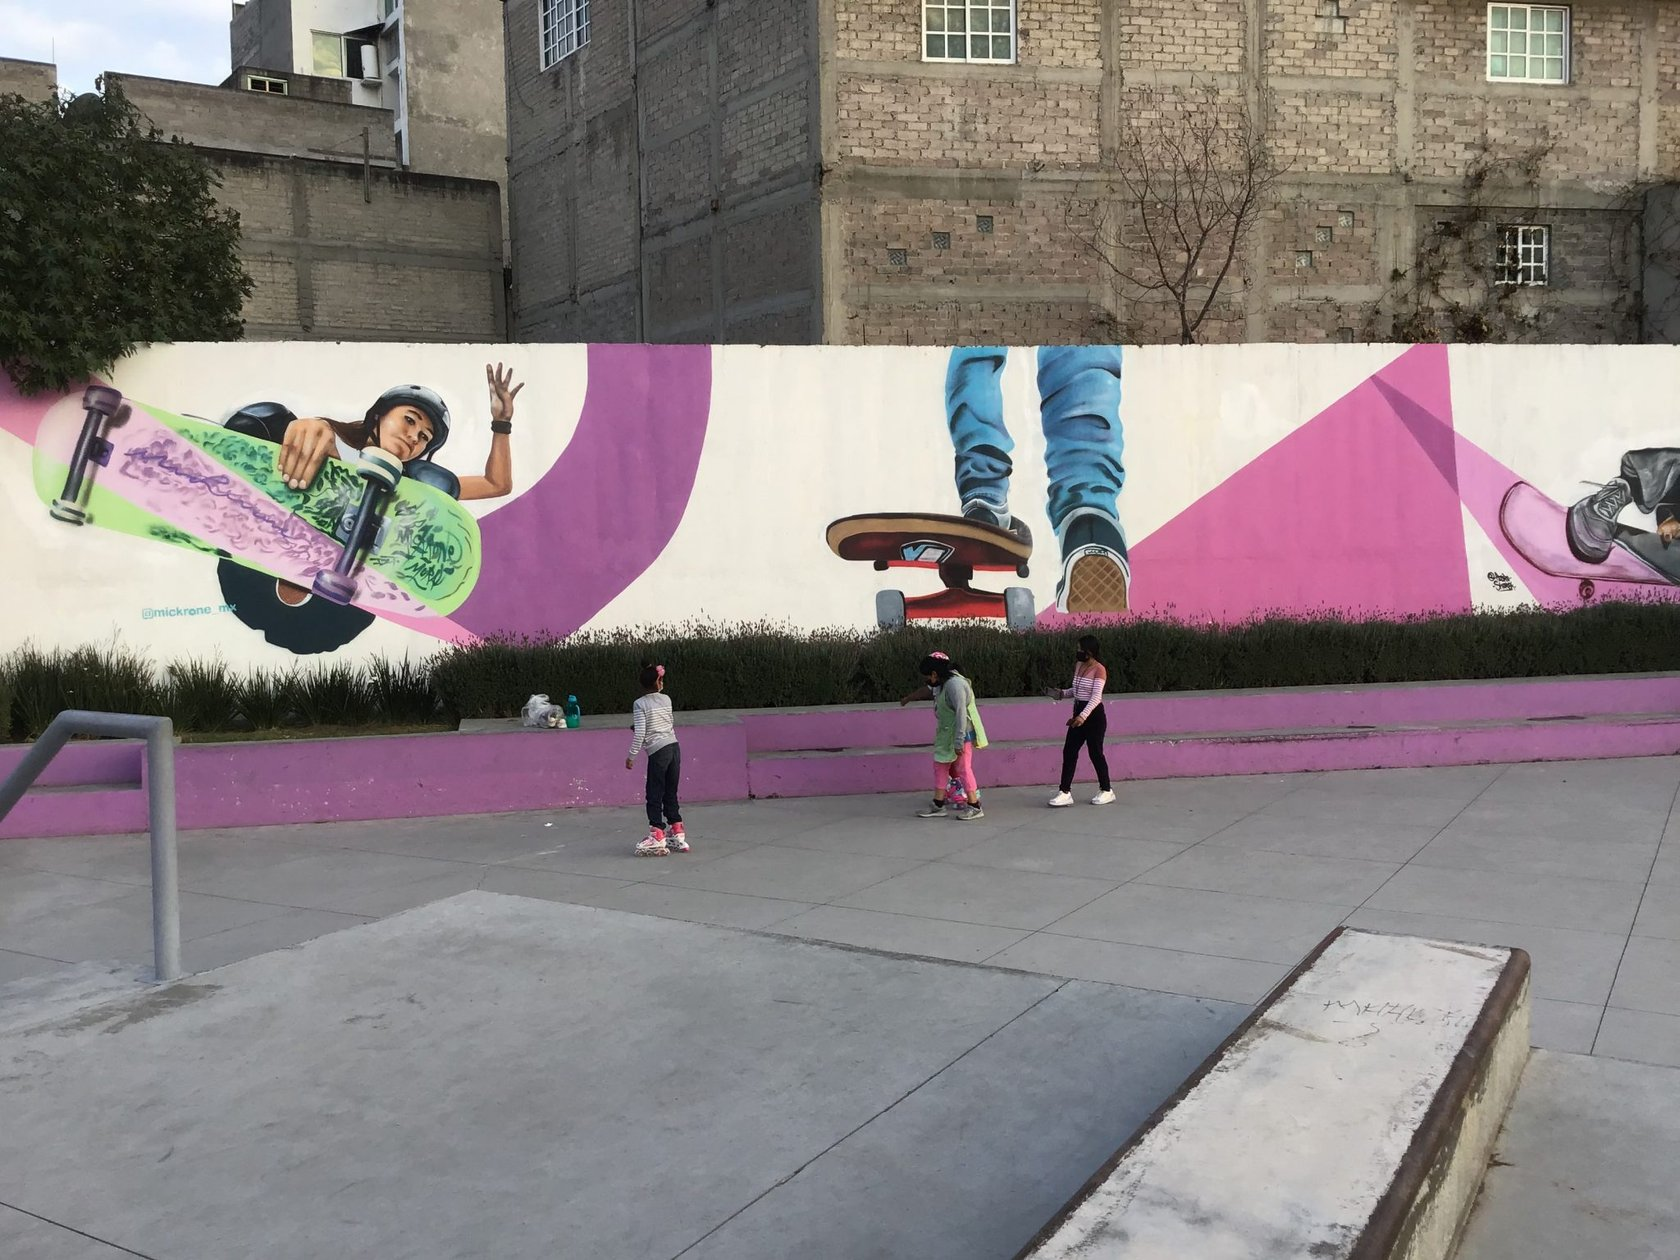
\includegraphics[width=0.7\textwidth]{images/IMG_8051-2048x1536.jpg}
\end{figure}

(1) Inclusion is a powerful tool in an integration effort; a public space doesn’t need to be heavily guarded nor regulated to feel safe if the dynamics are conducive to being used and enjoyed. Public spaces need to be designed with the specific purpose of serving the current needs of the community, instead of serving the ideal future projection of a community.

(2) People appreciate having a recreational space to spend time with their friends and family.  What’s more, offering proper management of these spaces can make them safer and more enjoyable.

(3) Finally, we learned that the cableway was an excellent choice of public transportation given both topographical and cultural circumstances – a topic for another day!

Significado:Atzintli (“Agua Chiquita”, “Agüita” o “Gota de Agua” en Náhuatl).

La Utopía Hídrica Atzintli:Espacio del Agua, recuerda a sus visitantes la vitalidad e importancia del agua, en particular por dos elementos diseñados para su captación, preservación y aprovechamiento en el Parque Hídrico La Quebradora y la vecina planta de tratamiento del Sistema de Aguas de la Ciudad de México.

En sus distintas fases como proyecto para la comunidad, éste espacio ha tenido un fuerte impulso por la sustentabilidad hídrica, y ha sido premiado a nivel internacional. Se localiza en la confluencia de colonias de la Sierra de Santa Catarina con altos índices de marginación, como Xalpa, Citlalli, Buenavista, Tenorios y Santa María Aztahuacán.

Actividades en Utopia Atzintli:Entre algunas de las Actividades y Espacios que podras disfrutar en la Utopia Atzintli se encuentran:

Clases de Natación \textasciitilde{} Gimnasio al Aire Libre \textasciitilde{} Yoga y Taichi

Multi-Canchas \textasciitilde{} Patinaje en Skate-Park \textasciitilde{} Pista de Tartán

Clases de Danza \textasciitilde{} Talleres de Música \textasciitilde{} Foro al Aire Libre

\begin{figure}[htbp]
  \centering
  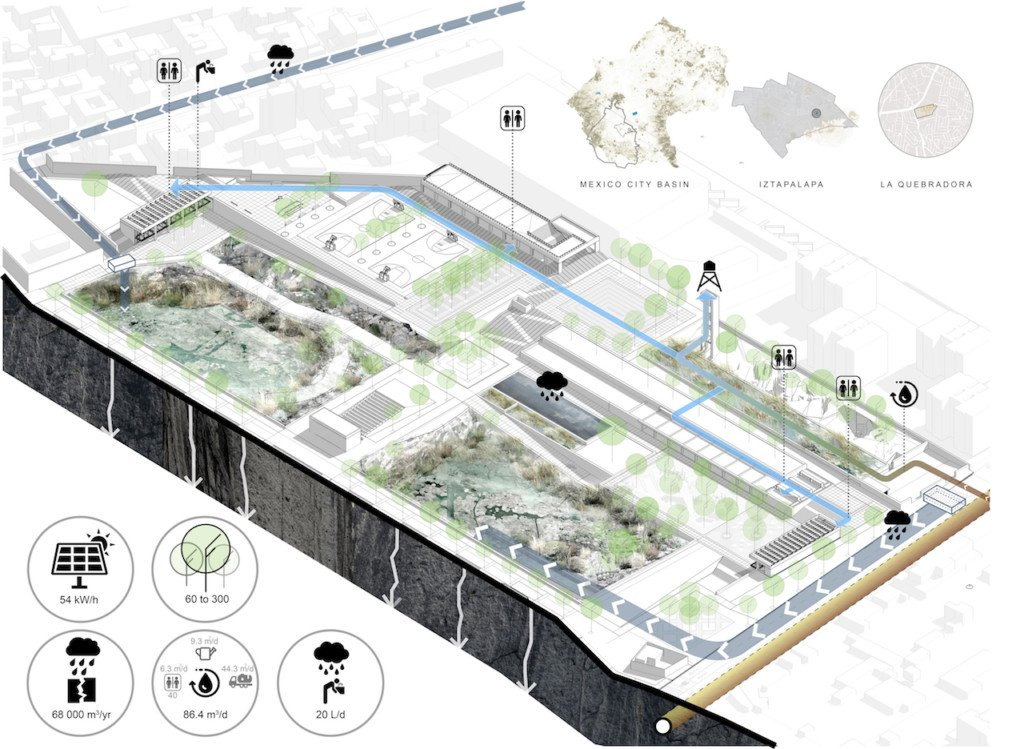
\includegraphics[width=0.7\textwidth]{images/18-arquine-castro-quebradora-1024x749-1.jpg}
\end{figure}

\vspace{2em}
\fbox{\parbox{\dimexpr\textwidth-2\fboxsep-2\fboxrule\relax}{
\raggedright
  \small This PDF was automatically generated using the Python-to-LaTeX tool available at~\url{https://github.com/Our-Greenway/scrape2TeX}.\\[0.5em]
  If there are any differences, the online version at~\url{https://www.ourgreenway.ca/once-we-get-there-a-plethora-of-parks-utopia-de-iztapalapa-atzintli} shall prevail.
}}
\end{document}